\subsubsection*{Kinetic Component (\ref{eqn:linearized Boltzmann equation})}
    The kinetic component comprises an inhomogeneously linear, conservative PDE in position space, $\bfx$, and velocity space, $\bfv$. Classical techniques for the numerical solution of conservative PDEs include:
    \begin{itemize}
        \item  Monte Carlo--like Lagrangian pseudo-particle techniques\footnote{To be able to derive a pseudo-particle model from such a kinetic equation, certain conditions must be satisfied by the collision operator. This will be discussed further in Section \ref{cha:collision operators}.}
        \item  Classical Eulerian techniques (FEM/FDM/etc.)
    \end{itemize}
    For these equations, the former particle-in-cell (PiC) approach has many benefits over classical PDE techniques: \BA{(Michael Barnes disagrees, so I'd be interested to hear his reasoning.)}
    \begin{itemize}
        \item  {\bf Particle decoupling from non-linearity:} Whereas in traditional PiC models, the pseudo-particles interact directly with one another through a distinct EM field---analogous to nonlinear collision operators in the Boltzmann equations (\ref{eqn:Boltzmann equation})---pseudo-particle techniques for the linearized Boltzmann equations require no such coupling, due to the equations' linearity. Particles interact indirectly \emph{through} the fluid component. (See Figure \ref{fig:PiC decoupling})

        This reduces the number of component-to-coupling information couplings from $\calO[n^{2}]$, in a classical direct PiC method, to $\calO[n]$, where $n$ is the number of particles in the pseudo-particle layer.
        
        \begin{figure}[!ht]
            \centering
            \begin{subfigure}{0.5\textwidth}
                \centering
                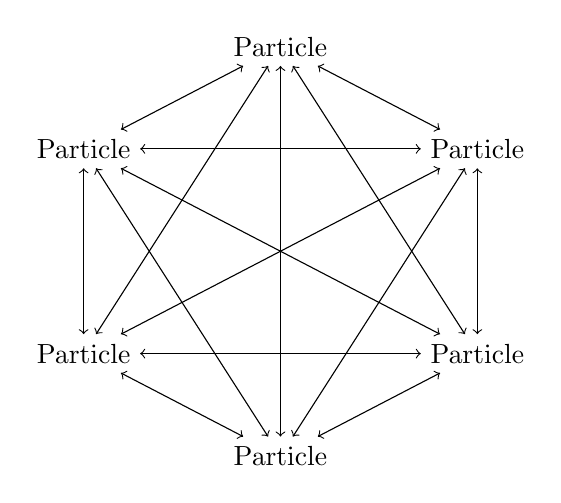
\begin{tikzpicture}[align = center, node distance = 4cm, auto]
                    \node (1) at (    0,   2.6) {Particle};
                    \node (2) at (  2.5,   1.3) {Particle};
                    \node (3) at (  2.5, - 1.3) {Particle};
                    \node (4) at (    0, - 2.6) {Particle};
                    \node (5) at (- 2.5, - 1.3) {Particle};
                    \node (6) at (- 2.5,   1.3) {Particle};
                    
                    \draw[<->] (1) -- (2);
                    \draw[<->] (1) -- (3);
                    \draw[<->] (1) -- (4);
                    \draw[<->] (1) -- (5);
                    \draw[<->] (1) -- (6);
                    
                    \draw[<->] (2) -- (3);
                    \draw[<->] (2) -- (4);
                    \draw[<->] (2) -- (5);
                    \draw[<->] (2) -- (6);
                    
                    \draw[<->] (3) -- (4);
                    \draw[<->] (3) -- (5);
                    \draw[<->] (3) -- (6);
                    
                    \draw[<->] (4) -- (5);
                    \draw[<->] (4) -- (6);
                    
                    \draw[<->] (5) -- (6);
                \end{tikzpicture}
                \caption{Coupling in a classical PiC method for the Boltzmann equations: $\calO[n^{2}]$}
            \end{subfigure}%
            \begin{subfigure}{0.5\textwidth}
                \centering
                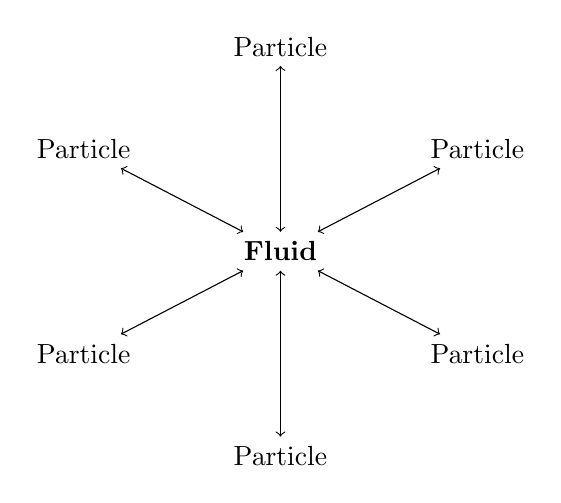
\begin{tikzpicture}[align = center, node distance = 4cm, auto]
                    \node (Fluid) at (0, 0) {\bf Fluid};
                    \node (1) at (    0,   2.6) {Particle};
                    \node (2) at (  2.5,   1.3) {Particle};
                    \node (3) at (  2.5, - 1.3) {Particle};
                    \node (4) at (    0, - 2.6) {Particle};
                    \node (5) at (- 2.5, - 1.3) {Particle};
                    \node (6) at (- 2.5,   1.3) {Particle};
                    
                    \draw[<->] (Fluid) -- (1);
                    \draw[<->] (Fluid) -- (2);
                    \draw[<->] (Fluid) -- (3);
                    \draw[<->] (Fluid) -- (4);
                    \draw[<->] (Fluid) -- (5);
                    \draw[<->] (Fluid) -- (6);
                \end{tikzpicture}
                \caption{Coupling when using a PiC model for the \\ correction in a $\delta\! f$ method: $\calO[n]$}
            \end{subfigure}
            \caption{Illustration of the how the coupling between the model components (fluids/patricles) differs when using a PiC correction vs. a classical PiC model. \BA{(Would like an extension of this diagram when I talk about approaches for and difficulties in parallelisation later too.)}}
            \label{fig:PiC decoupling}
        \end{figure}
        
        \item  {\bf Infinite velocity domain:} Lagrangian techniques are preferable under such conditions since---while classical Eulerian techniques for the solution of PDEs over infinite velocity domains exist \BA{[Ref, Ref, ....]}---Lagrangian techniques require no separate decision and analysis, which can often be relatively arbitrary.

        \item  {\bf Non-local collision operators:} Hand-in-hand with the advantages for infinite velocity domains comes the advantages posed by PiC methods for linearized (local) collision operators, $\partial\bfC_{\pm_{1}\pm_{2}}^{(0)}$, that are non-local in velocity space, $\bfv$. Due to their ability to model both small- and large-angle collisions, non-local collision operators, such as fractional Laplacian models \cite{Cho_2015, Sakomoto_2016, Kiselev_Schmalian_2019} or those derived directly from the molecular chaos hypothesis from classical kinetic theory \cite{Lerner_Trigg_1991}, serve some of the most fundamental and accurate collision operator models in thermodynamics. \BA{(Good place for a little literature review on non-local/fractional Laplacian collision operators.)}
        
        Non-local terms pose a huge problem for traditional Eulerian PDE techniques, which rely on the PDE's locality for the creation of sparse, parallelizable matrix solves. This is not a problem for particle models, however, where the non-locality simply leads to occasional larger changes in the pseudo-particle velocities.

        By way of example, consider the following fractional PDE for a reduced (spatially-homogeneous, non-dimensionalized) kinetic model in $f(v; t)$, where $v  \in  \bbR$ is 1-dimensional, for some $\alpha  \in  (0, 2]$:
        \begin{equation}
            \partial_{t}f  =  \sqrt{|\Delta_{v}|}^{\,\alpha}f
        \end{equation}
        This is the Fokker Planck--type PDE satisfied by the probability density function of a normalised 1D Lévy flight with stability parameter $\alpha$. Its solution can therefore be modelled numerically through the use of a collection of pseudo-particles $V_{i}(t)$, each moving according to the same normalised 1D $\alpha$--Lévy flights. Examples of such flights for $\alpha  \in  \{1.1, 1.5, 2.0\}$ are shown in Figure \ref{fig:Levy flight examples}. \BA{(How non-local collision operators manifest for the particle SDEs.)} \BA{(Talk about how lower $\alpha$ values have larger jumps, manifested through the non-existence of $< \alpha$ moments.)}

        \begin{figure}[!ht]
            \centering
            \includegraphics[width = 0.8\textwidth]{1 - low-noise PiC models/2 - FEM vs PiC coupling/2 - PiC/images/Levy flight examples.png}
            \caption{Examples of normalised 1D Lévy flights for stability parameters $\alpha  \in  \{1.1, 1.5, 2.0\}$. Note the increased frequency of large jumps for smaller values of $\alpha$. (Source: \cite{Ai_Shao_Zhong_2012})}
            \label{fig:Levy flight examples}
        \end{figure}
        
        \item  {\bf Regions of high and low thermalization:} Pseudo-particle methods need only model the function where it is non-zero. Similarly, for functions that exhibit certain regions of comparatively large and small values, pseudo-particle methods can inherently focus more computational processing power to those regions of larger value, and less to those regions of smaller value.
        
        For plasmas, one might expect different regions where the plasma:
        \begin{itemize}
            \item  Largely thermalized and kinetic effects are \emph{less} prominent, i.e. where $f_{\pm}$ are \emph{closer} to $f_{\pm}^{(0)}$ and $\delta\! f_{\pm}$ are correspondingly \emph{smaller} (e.g. in the plasma core).
            \item  Further from thermalization and kinetic effects are \emph{more} prominent, i.e. where $f_{\pm}$ are \emph{further} to $f_{\pm}^{(0)}$ and $\delta\! f_{\pm}$ are correspondingly \emph{larger} (e.g. close to a beam injection device, or near the reactor walls).
        \end{itemize}
        Pseudo-particle methods can use this to their computational advantage, where classical PDE techniques cannot.
    \end{itemize}

    \BA{Why PiC for correction?
    \begin{itemize}
        \item  Good choice of collision operators leaves a parabolic PDE which can be simulated using Monte Carlo-like pseudo-particle SDEs that pop into and vanish from existence as time progresses, which are (unlike traditional PiC methods that \emph{don't} use the thermalized background) entirely decoupled. (Give example of such operators---e.g. Bhatnagar--Gross--Krook (BGK) \cite{Bhatnagar_Gross_Krook_1954}/Lénard--Bernstein (should ask Paul Dellar for a reference here)---but wait till the kinetic component chapter before fully classifying them.) This has 2 benefits:
        \begin{itemize}
            \item  Workload goes from $\calO[n^{2}]$ to $\calO[n]$:- diagram of star-like network showing coupling of fluids with each particle individually instead of all particles together.
            \item  Can use gyroaveraging with far less concern. Very easy to gyroaverage an SDE in fact.
        \end{itemize}
    \end{itemize}}
    